\section{Descrizione del sistema}\label{Descrizione del sistema}

\subsection{Materiale utilizzato}

Per il progetto sono state utilizzate:
\begin{enumerate}
    \item una MPU-6050 a 6 gradi di libertà (3\textit{dof accelerometer} + 3\textit{dof gyroscope});
    \item due MPU-9250 a 9 gradi di libertà (3\textit{dof accelerometer} + 3\textit{dof gyroscope} + 3\textit{dof magnetometer});
    \item un multiplexer TCA9548A (per permettere l'utilizzo di più IMU sullo stesso canale I2C);
    \item una scheda ESP32 programmabile con Arduino.
\end{enumerate}

\begin{figure}[H]
    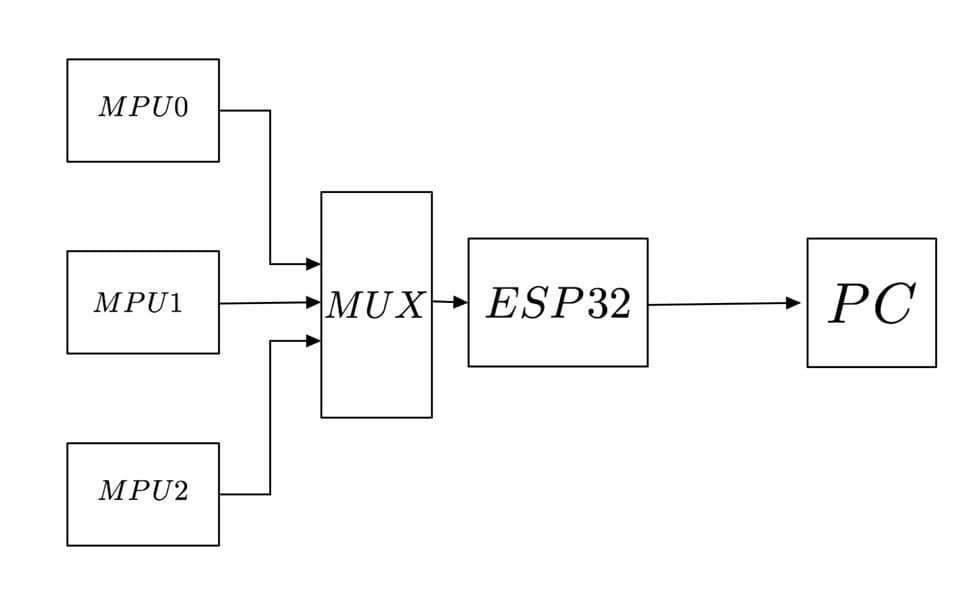
\includegraphics[scale=0.35]{immagini/schema_blocchi.jpg}
    \centering
    \caption{Schema a blocchi complessivo.}
\end{figure}

\clearpage

\subsection{Caratterizzazione IMU}\label{Caratterizzazione IMU}

Una IMU è un'unità di misura inerziale che comprende tre accelerometri e tre giroscopi posti sui tre assi di interesse dell'IMU (assi \textit{body}).

\subsubsection{Dati accelerometro}\label{Dati accelerometro}

\begin{figure}[H]
    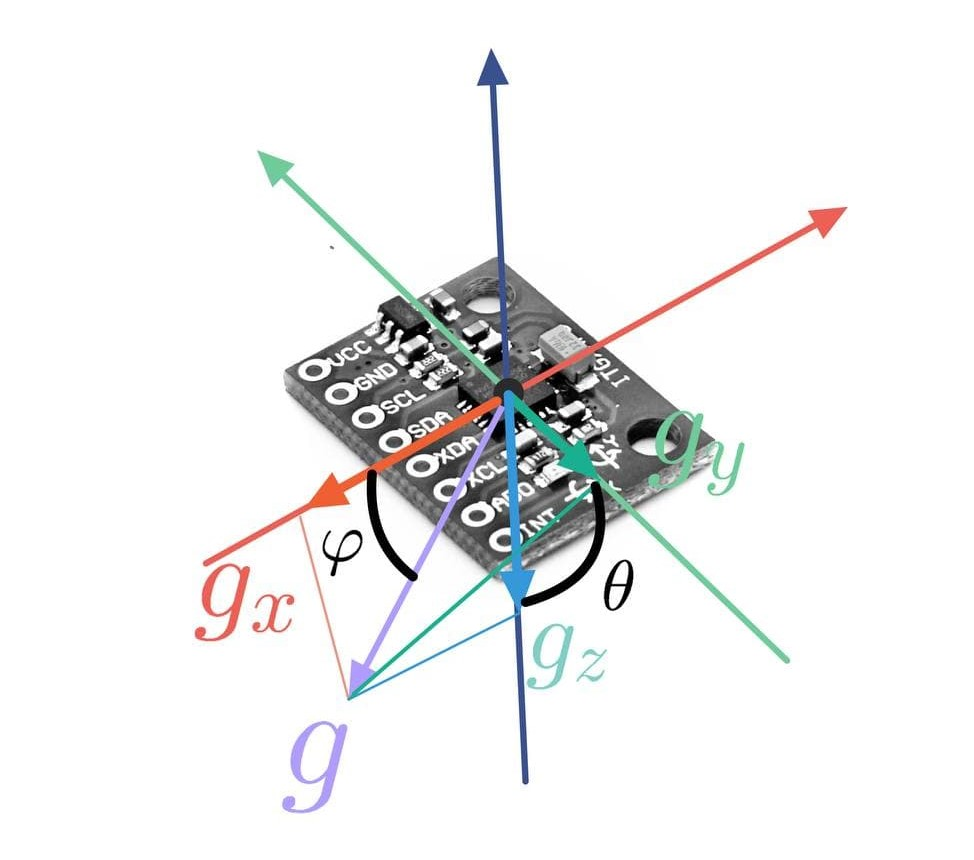
\includegraphics[scale=0.35]{immagini/IMU_sdr_g.jpg}
    \centering
    \caption{Accelerometro.}
\end{figure}

Attraverso i dati dell'accelerometro, si può inferire l'inclinazione di roll (rotazione attorno all'asse x) e pitch (rotazione attorno all'asse y) dell'IMU, considerando i valori trovati sui tre assi locali (\textit{body}) come le componenti parziali del vettore gravità, che sappiamo puntare verso il basso in assi fissi (\textit{navigation}).

\begin{equation}\label{eq phi roll acc}
    \phi_a = \tan^{-1} \begin{pmatrix} \frac{a_y}{a_z} \end{pmatrix}
\end{equation}
\begin{equation}\label{eq theta pitch acc}
    \theta_a = \tan^{-1} \begin{pmatrix} \frac{-a_x}{a_y \sin{\phi_a} \, + \, a_z \cos{\phi_a}} \end{pmatrix}
\end{equation}

D'altra parte, usare solo le misure date dagli accelerometri genera errori nel caso in cui l'IMU, invece che venire ruotata, sia sottoposta a un'accelerazione data da un moto lineare: in tal caso, questo metodo riporterebbe rotazioni che non esistono. Per questo è necessario filtrare le misure con altri sensori, in modo che gli errori di uno vengano compensati dagli altri (la cosiddetta \textit{sensor fusion}).

\clearpage

\subsubsection{Dati giroscopio}\label{Dati giroscopio}

\begin{figure}[H]
    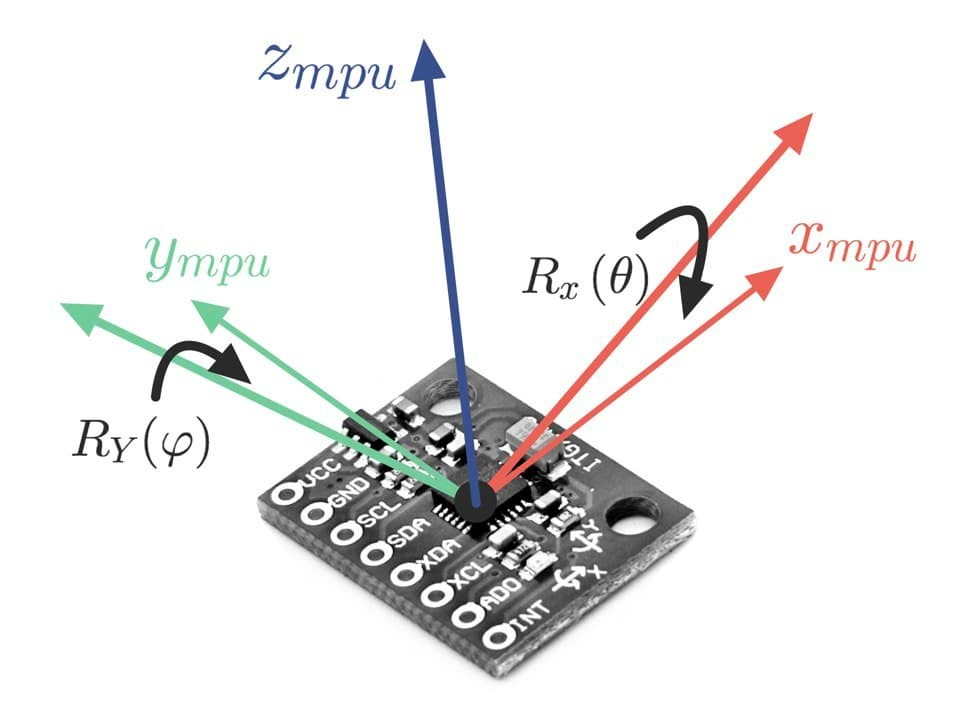
\includegraphics[scale=0.25]{immagini/IMU_sdr_R.jpg}
    \centering
    \caption{Giroscopio.}
\end{figure}

Allo stesso modo dell'accelerometro, il giroscopio può trovare la velocità angolare sui tre assi di riferimento. In questo caso, una semplice operazione di integrazione ci consente di ricavare gli angoli relativi nel tempo, che poi vengono sommati alla loro misura precedente.\\
Questo metodo necessita la conoscenza dell'orientazione iniziale dell'IMU, ma tale richiesta viene soddisfatta ponendo gli angoli iniziali a 0 e facendo partire il programma che invia i dati quando il guanto è parallelo al suolo (roll e pitch nulli).

\begin{equation*}
    \dot{q}_{gyro} = \frac{1}{2} \, \Omega_t \, q
\end{equation*}
\begin{equation*}
	q_{gyro} = q + \dot{q}_{gyro} \, dt
\end{equation*}\label{integr gyro}

\begin{figure}[H]
    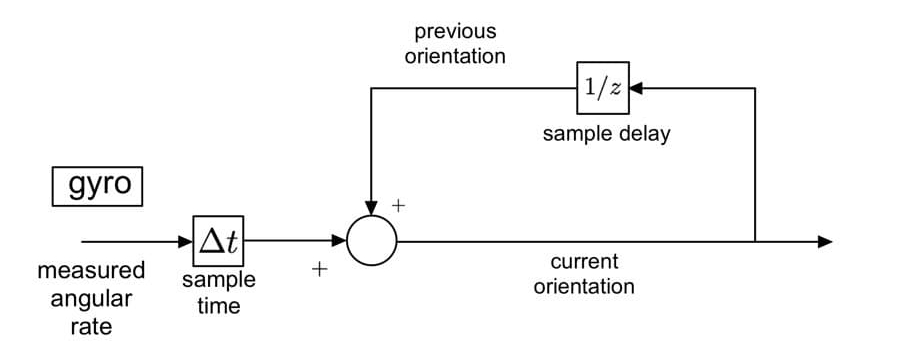
\includegraphics[scale=0.35]{immagini/photo_2022-03-07_09-40-18.jpg}
    \centering
    \caption{Elaborazione dati giroscopio.}
\end{figure}

Per l'integrazione delle misure delle velocità angolari, sono state usate le formule (\ref{integr phi}), (\ref{integr theta}) e (\ref{integr psi}), che combinano sia la semplice operazione di integrazione con una rotazione rispetto agli angoli dello step precedente, in modo che i sistemi di riferimento tra angoli trovati con accelerometro-magnetometro e giroscopio siano allineati.

\begin{equation}\label{integr phi}
    \dot{\phi} = p + q \sin{\phi} \tan{\theta} + r \cos{\phi} \tan{\theta}
\end{equation}

\begin{equation}\label{integr theta}
    \dot{\theta} = q \cos{\phi} - r \sin{\phi}
\end{equation}

\begin{equation}\label{integr psi}
    \dot{\psi} = q \sin{\phi} \sec{\theta} + r \cos{\phi} \sec{\theta}
\end{equation}\\

Un problema più grave invece è la considerazione dell'errore del giroscopio nel tempo: poiché la misura della velocità angolare è sottoposta a rumore, integrare tale misura contribuisce al \textit{drifting}, ovvero una forma di alterazione della misura in cui l'angolo ricavato aumenta nel tempo anche se l'IMU rimane ferma.\\
Per risolvere il \textit{drifting} si usa la misura ricavata dall'accelerometro come correzione.

\clearpage

\subsection{Caratterizzazione AHRS}

Un AHRS (talvolta chiamato MARG per \textit{Magnetic, Angular Rate and Gravity}) è un sistema di riferimento di orientazione e direzione che include una IMU e un magnetometro.\\
In particolare, le MPU-9250 usate hanno come base un'IMU uguale alle MPU-6050 a cui è stato aggiunto un magnetometro AK8963 a 3 gradi di libertà.

\subsubsection{Dati magnetometro}\label{Dati magnetometro}

\begin{figure}[H]
    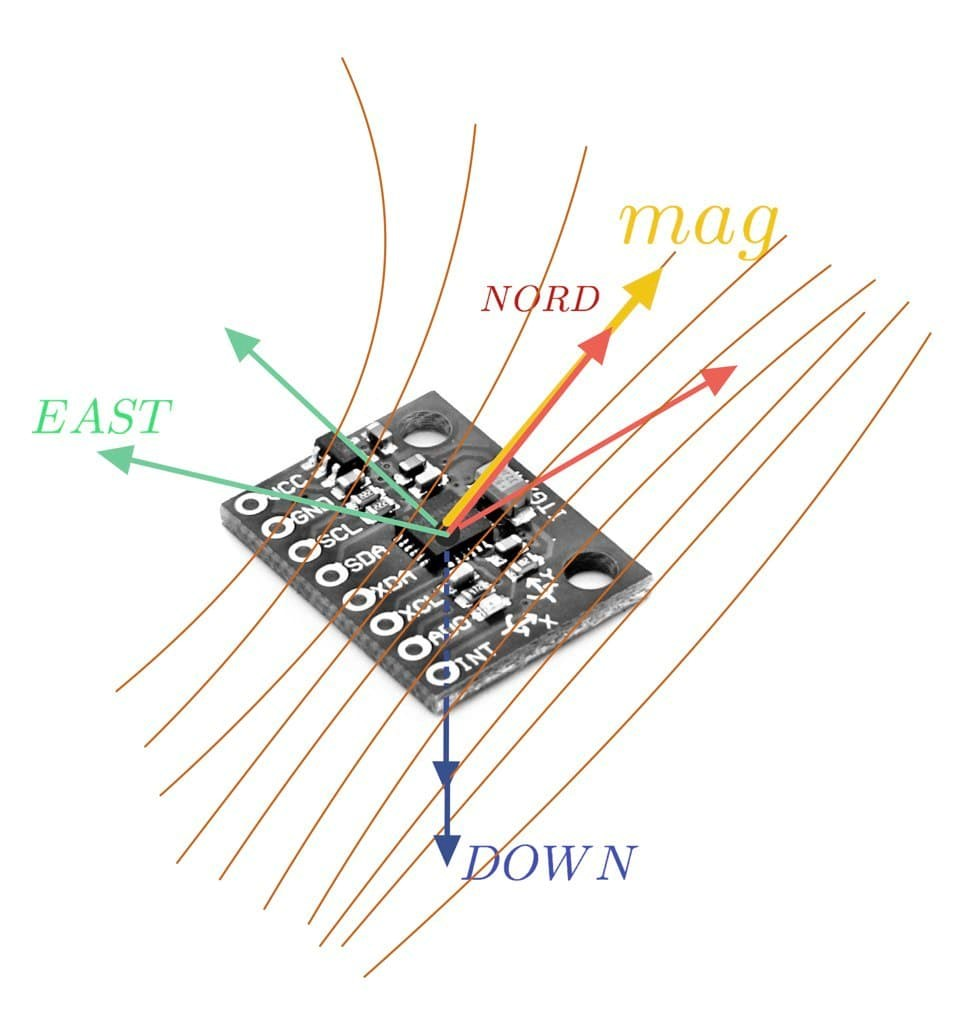
\includegraphics[scale=0.25]{immagini/IMU_sdr_magn.jpg}
    \centering
    \caption{Magnetometro.}
\end{figure}

Nelle AHRS ad accelerometro e giroscopio delle IMU si aggiunge la misura di \textit{heading} data dal magnetometro, che permette di ricavare anche lo yaw (rotazione attorno all'asse z) del dispositivo.\\

I passaggi sono i seguenti: si ruotano i dati ricevuti dal magnetometro ($m$) utilizzando i valori di roll e pitch già ricavati dall'accelerometro, e da essi si ricava lo yaw.
\begin{equation*}
    \begin{bmatrix} b_x\\ b_y\\ b_z \end{bmatrix} = R_y(\theta_a) R_x(\phi_a) \begin{bmatrix} m_x\\ m_y\\ m_z \end{bmatrix}
\end{equation*}
\begin{equation*}
    \psi_m = \tan^{-1} \begin{pmatrix} \frac{-b_y}{b_x} \end{pmatrix}
\end{equation*}
Da cui risulta
\begin{equation}\label{eq psi yaw magn}
    \psi_m = \tan^{-1} \begin{pmatrix} \frac{m_x \sin{\phi_a} \, - \, m_y \cos{\phi_a}}{m_x \cos{\theta_a} \, + \, m_y \sin{\theta_a} \sin{\phi_a} \, + \, m_z \sin{\theta_a} \cos{\phi_a}} \end{pmatrix}
\end{equation}

\clearpage

\subsection{Posizionamento delle IMU}

\begin{figure}[H]
    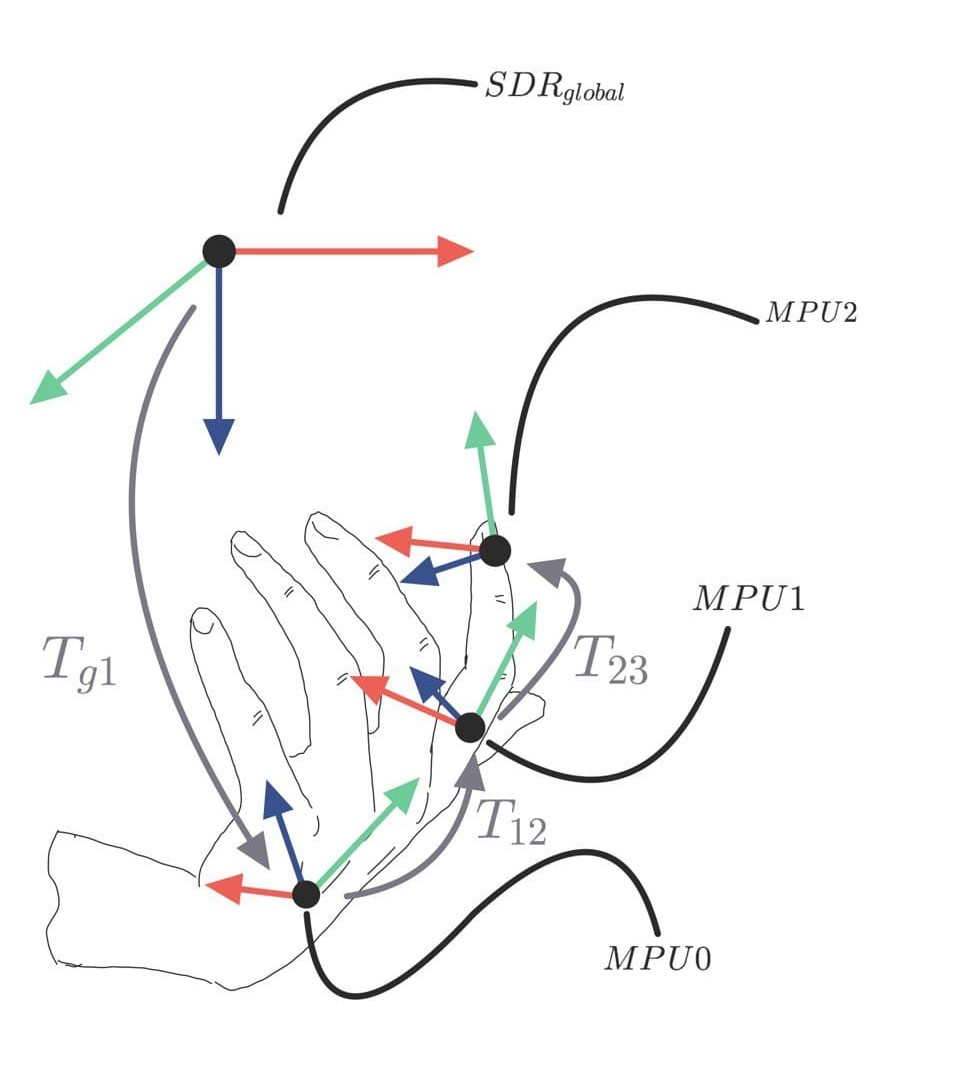
\includegraphics[scale=0.25]{immagini/guanto_sdr.jpg}
    \centering
    \caption{Sistemi di riferimento del dito.}
\end{figure}

Le MPU-9250, essendo provviste di magnetometro per misurare l'\textit{heading}, sono state poste una sul dorso della mano (MPU0), per poterne visualizzare lo yaw, e una sulla falange prossimale, ovvero quella più vicina al palmo (MPU1), in modo da poter visualizzare rotazioni relative tra il dito e il palmo della mano. La MPU-6050 è stata invece posizionata sulla falange distale, ovvero quella più vicina alla punta del dito (MPU2).\\

\begin{figure}[H]
    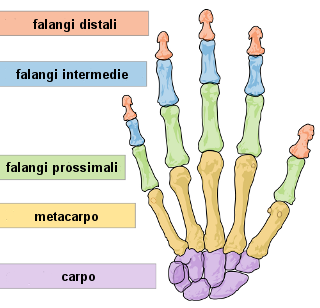
\includegraphics[scale=0.45]{immagini/falangi.png}
    \centering
    \caption{Falangi di una mano.}
\end{figure}

\clearpage